% !TeX root = ../main.tex
% !TeX spelling = en_GB
% !TeX program = pdflatex

\chapter{Discussion}
\label{chap:discussion}

This chapter includes an extends the discussion of the result mainly published in Paper III, also included here in \Cref{chap:results}. It also includes a discussion about the initial choice of method and some details that are not fully covered in the attached papers. 

The chapter begins with a discussion on the systematic difference noticed between the \gls{cdp} and the \gls{dii}. It continues with a reflection on the two \gls{nwp} model resolutions used. 

After this, there is a section about some of our first questions regarding lighting and imaging of small particles, a section on the image noise and a description of some difficulties that was encoutered during the size measurement verification using polymer microspheres. The use of LED light and the measurement accuracy based on statistical data are discussed. 

Finally, the droplet size, the sampling speed (including the measurement volume) and the \gls{dsd} are discussed.


\section{Cause of Systematic Difference}
\label{sec:systemdiff}

The measured LWC of the DII and the CDP in Figure \ref{fig:0228-0301_LWC_DIIvsCDP} differs by a factor of approximately 3.65 (CDP LWC / DII LWC). There may be several reasons for this difference.

Comparing the measured MVD of the DII and the CDP we get a quote between the two instruments of 0.77. This means that the MVD of the CDP is on average 30 percent higher than the DII. Since the LWC is proportional to the third power of the droplet size, an increase in the diameter of 30 percent will increase the LWC by $1.3^3=2.2$. Unless the droplets are affected by the instruments themselves, there are two possible explanations. One is that the two instruments measure the sizes of the droplets differently. The other is that the sampling volume differs depeding on the size of each droplet for one or both instruments.

The CDP and its predecessors, have shown a tendency of oversizing droplets when calibraded by glass or polymer spheres \cite{wend1996,lance2010}. This could still explain some of the difference. The precision of the CDP size measurement is also limited by the fixed size bins, and by the pulse amplitude of the scattered light calculated from Mie theory \cite{lance2010,bohr2008}. A small disturbance, like a slight misalignment of the laser beam, may cause a shift in the optical response pushing the size to the next or previous size bin \cite{lance2010}. The sampling area, i.e. the illumninated area that the particles must pass through to be recorded, is an average value given by the manufacturer on delivery. 

From Figure \ref{fig:0228-0301_WSvslwcquote} we conclude that there is no relation between the difference between the two instruments and the wind speed when the wind speed is below four meters per second.

The LWC value depends on an accurate estimation of the sampling volume. While the image area can be determined accurately, the measuring range depends both optical factors and the image processing and segmentation. The measuring range depends e.g. on the light exposure. It may also depend on the distance from the object to the optical center. Since the calibration of the measurement range was only done once, close to the optical center, the sampling volume of the DII may actually be smaller than estimated. How much smaller? Dividing the image area in segments and make a calibration in each segment would give the answer.

\section{Model Data}

By comparing the results from 11. December with other dates, it seems that the high resolution gives values of LWC that are close to the measured, while the low resolution gives a LWC that indicates fog, but fails to accurately predict the amount or the time of occurrence. To predict icing at a particular location, the 500 m model resolution gives better agreement than the 2.5 km resolution. It is likely that the difference is caused by the complex topography at and around the measurement site.

\section{Starting Studies}
\label{sec:discussionstarting}

The feasability study of different illumination wavelengths and coherent lighting, the result from the measurement of energy required for image exposure and the influence of ambient light on the measurement is discussed.

\subsection{Infrared and Visible Light}

The amount of absorbed light in a small water droplet is close to negligible compared to the scattered light. In a large ensemble of droplets, such as a cloud, the total absorption will still be significant, especially for wavelengths in the near and far infrared. We had the opportunity to make a quick comparison of illumination using blue light (ca 450nm) and near infrared (ca 850nm). The blue light gave the sharpest image; possibly because of the higher theoretical resolving power as described by Rayleigh's criterion. But it might also partly be explained by the difference in the sensor's sensitivity for the different wavelengths. See Paper I.

\subsection{Laser Light}
\label{sec:discussionlaser}

Lasers are used in numerous optical instruments for droplet measurement, and there is good reason to. Prices for high power semiconductor lasers have become very attractive. With a laser it is possible to achieve a short light pulse with high energy. The coherency causes strong diffraction patterns, something that is used when reconstructing images in holographic imaging instruments This makes it possible to achieve a larger measuring range than what is possible in conventional imaging, as mentioned in section \ref{sec:relwork}.
 
Laser illumination was tried using two wavelengths, 450 and 850 nm, and placed in different positions. \Cref{fig:laser} shows an example image with a 450 nm laser placed about 135 degrees from the optical center. Direct size and concentration measurement is difficult for at least following reasons: 
\begin{enumerate}
\item The measurement volume is difficult to define because the laser light intensity is spatially inhomogenous.
\item The light intensity in the measurement point is difficult to control. Overexposure makes the glare appear larger.
\item Interference patterns from particles outside the measurement volume is disturbing the measurement.
\end{enumerate}

\begin{figure}%[ht]
\centering\includegraphics[width=0.6\linewidth]{figures/450nm45deg_new}
\caption{Reflections and interference patterns by droplets in 450nm laser light. The light source is placed at a position about 135 degrees from the optical center.}
\label{fig:laser}
\end{figure}

For conventional imaging of small particles the coherence mainly causes problems. Although it is possbile to make the laser incoherent e.g. by using diffusers or optical fibres, it is just one of the things that makes the complete system slightly more complex.
%
%\subsection{Exposure Energy Measurement}
%\label{sec:expmeasurement}
%
%The measurement is also described in Paper I. The result is shown in \Cref{fig:expenergy}. The energy was measured by using a thermal power sensor, the area of view and the time that is required for a full exposure. 34 nJ is required for the area in view (7.8 $mm^2$) for the lowest gain setting, which results in the highest SNR and about 20 nJ for the used setting.
%
%\begin{figure}[ht]
%\centering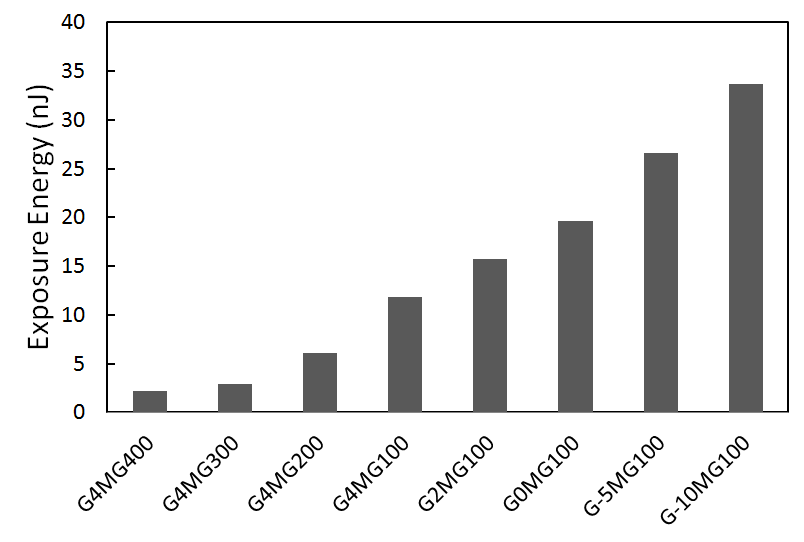
\includegraphics[width=0.75\linewidth]{figures/Energy_per_gain_level2}
%\caption{Light energy ($nJ$) for exposure in each of the eight gain levels used. The energy was tuned manually up to a level of high exposure, but not saturating any point in the image.}
%\label{fig:expenergy}
%\end{figure}

\subsection{Ambient Light}

The shortest possible exposure time according to the camera specification is 0.038 ms, slightly depending on other camera settings. For each measurement 152 images were captured, with an increasing exposure time from ca 0.04 to 1.99 ms. A delay of 1 second was set between each image. \Cref{fig:ambientlight} shows the mean pixel value and the standard deviation of the value for one of the measurements at 22000 lux ambient light.

\begin{figure}%[ht]
\centering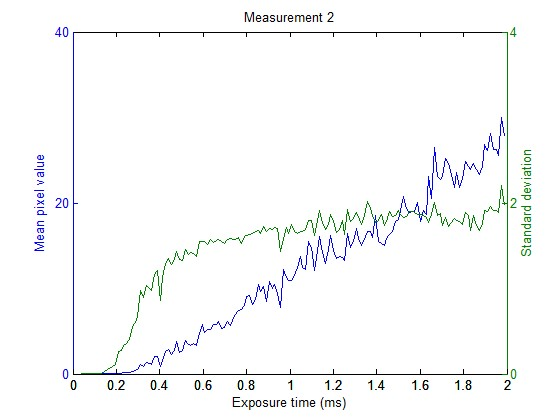
\includegraphics[width=0.6\linewidth]{figures/Amblight22000lux}
\caption{Mean pixel value and standard deviation of ambient for a light measurement at 22000 lux.}
\label{fig:ambientlight}
\end{figure}

Using this setup it was found that an exposure time of at least one second is needed to give a signal that is comparable to the noise level under normal exposure. At the same time, in order to image small droplets, the exposure time needs to be less than one μs. Therefore we concluded that the ambient daylight would likely have no effect on the measurement.

\section{Image Noise and SNR}
\label{sec:discnoise}
We observed a correlation between the \gls{snr} and the corresponding measuring range in Paper I. A higher \gls{snr} results in an increased measuring range. Even though the \gls{snr} is measured for every droplet, a compensation is not yet implemented for this. However, as was illustrated in Paper I, a higher \gls{snr} can be achieved by increasing the light intensity. Consequently, the sampling volume for every image could be increased by incresing the light intensity. 

The \gls{snr} for a ten micrometer dot image was calculated using seven gain level settings of the image sensor. For each gain level, the illumination time was adjusted so that the level of exposure was the same. This measurement was done using both the 455 and the 850 nm illumination. The result can be seen in \Cref{fig:noisegain}. Lower gain levels require longer light pulses, but results in higher \gls{snr}. It can also be seen that the \gls{snr} for 455 nm is systematically higher than for 850 nm. 

\begin{figure}%[ht]
\centering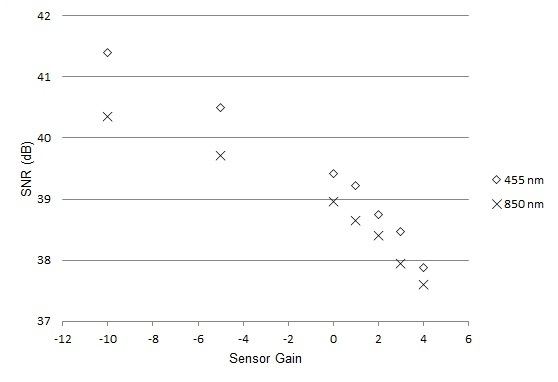
\includegraphics[width=0.6\linewidth]{figures/NoiseGain}
\caption{SNR for a ten micrometer dot image using two wavelengths and seven gain level settings. Shorter wavelength and lower gain gives less noise.}
\label{fig:noisegain}
\end{figure}

The design using a weakly collimated LED that illuminates an area slightly larger than the field of view makes the system quite insensitive to misalignment of the camera and the light source. Temporal or permanent changes in light intensity caused by a minor misalignment can be automatically compensated for by continuous measurement of the total exposure level. If the level of exposure increases or decreases, the length of the light pulse is changed correspondingly. The light intensity can also be affected by dirt on the front glass of the housings. 

Spatial dissimilarities in the light intensity that are not caused by noise can be compensated for by calculating the local average intensity of the background around each measured droplet. The size of a droplet is then based on the intensity dip, or modulation in amplitude, caused by the shadow compared with its local background noise, as illustrated in \Cref{fig:snrcalc}.

\section{Aerodynamics}

Many existing instruments suffer from errors caused by the instrument itself during sampling, e.g. when droplets get stuck on the inlet or shatters into smaller droplets. The DII is not as small and aerodynamically shaped as the \gls{cdp}, therefore a difference between the instruments would be expected depending on the air speed. However, a comparison between the measured values of LWC showed no correlation between the wind speed and the difference in the measured LWC. The wind speed during the comparison was only 1-4 $\mathrm{m \cdot s^{-1}}$, which probably explains why the less aerodynamic shape of the DII compared with the \gls{cdp} has no noticeable effect. This could change dramatically when measuring at higher wind speeds.

\section{Difficulties in the Polymer Microspheres Measurement}

To verifiy the sizing algorithm, a measurement using polymer microspheres of four known calibrated size distributions was done. To simulate real conditions as far as possible the microspheres were applied using the same dispenser used for the calibration of the \gls{cdp}. The smallest microspheres had a tendency of clogging, sometimes leading to a measurement of a clog as a single particle. Therefore all images were visually checked for false measurements. The outliers caused by false measurements were removed.

\subsection{Clogging of Microspheres}

Small microspheres form larger clogs that are measured as single microspheres. The reason may be static electricity or humidity. As was seen in the measurement of five micrometer spheres, the result of some clogs becomes outliers in the expected distribution. An example is shown in \Cref{fig:5umclog}. This needs to be considered when solid microspheres are used as reference objects. Colliding liquid water droplets would of course coalesce into larger droplets, thereby changing the diameter.

\begin{figure}[ht]
\centering\includegraphics[width=0.6\linewidth]{figures/5um_clogs}
\caption{An example showing an image of clogs of five micrometer microspheres. One of the clogs are measured as a single particle, since it is round enough for the roundness qualifying criteria.}
\label{fig:5umclog}
\end{figure}

The equipment and the dispenser was thoroughly cleaned using compressed air between each measurement. Still, microspheres or other contaminations could remain, changing the distribution slightly.

Measured mean and standard deviation of all distributions were found to be within the stated calibrated values. This can be seen as a confirmation that the instrument calibrated only by the micrometer dot scale measures the microsphere samples correctly.

\subsection{Roundness}

A perfectly circular disc measured using an infinite resolution would have an expected roundness value equal to one. In practice, this is not possible to achieve in a digital image. But the contour is only used as detection criteria. Instead, the diameter is calculated using the negative shadow intensity. Therefore the contour roundness itself should have no great impact on the accuracy.

The roundness criteria defined in section \ref{met:roundness}. The roundness (\ref{eq:5}) limit set at 0.85 in this measurement, seems to work fine. It excludes most irregular objects, like clogs in the five micrometer measurement. When measuring fogs in cold climates, the water droplets will be mixed with ice crystals. While larger crystals will mostly be sorted out by the roundness criteria, crystals smaller than ten micrometer could present a challenge, and five micrometer ice crystals are more or less impossible to distinguish from liquid water droplets, unless they are very different in shape.

\begin{figure}[ht]
\centering
\begin{subfigure}[t]{.5\textwidth}
  \centering
  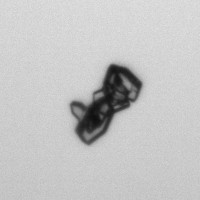
\includegraphics[width=1\linewidth]{figures/litenis1}
  \subcaption{Ice particle.}
  \label{fig:litenis}
\end{subfigure}%
\begin{subfigure}[t]{.5\textwidth}
  \centering
  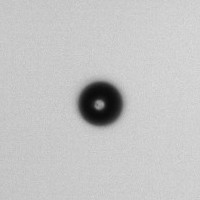
\includegraphics[width=1\linewidth]{figures/litendroppe1}
  \subcaption{Droplet.}
  \label{fig:litendroppe}
\end{subfigure}
\caption{Difference between an ice particle and a water droplet that is 62 µm in diameter. Larger ice and snow particles tend to be more complex in shape. Ice particles smaller than 10 µm in diameter may be difficult to distinguish from water droplets.}
\label{fig:icevsdrop}
\end{figure}

\subsection{Calibration Validation}

The calibration functions derived from the measurement of known-sized dots is an approximation and an interpolation. It is assumed that light scatters similarly on the edge independently of the size of the object. However, this is not quite true, especially for smaller particles \cite{bohr2008}. For particles around ten micrometer or less in diameter we would expect a diffraction pattern with intensity variations. The pattern would be stronger the more coherent the illumination and more dominant the smaller the particle. In this system, using LED illumination, the coherence length is so short that no diffraction patterns are directly visible. This may also be explained by limitations of the optical resolution. Still changes to the edge for the smallest diameters cannot be entirely ruled out.

The experiment using calibrated spheres described in Paper II, confirmed that the measurement of droplet diameters was accurate. It was, however, not a confirmation of the measurement volume, since we did not know the concentration of microspheres. This was done using the \gls{cdp} as described in Paper III.

\section{LED Illumination}
\label{sec:ledillumination}
Using a high power LED instead of laser reduces the interference effects used in e.g. holography \cite{henn2013}, but since it is a monochromatic source, interference could not be completely ruled out. The coherence length for the blue LED is calculated in Paper I.

One would expect diffraction patterns depending on the spectral bandwith of the light source. The narrower the bandwidth, the stronger the diffraction. A spectrum analysis of the \gls{led} showed that the coherence length of the blue \gls{led} is about 6.8 μm. Therefore the spectrum was measured using a spectrum analyzer. The result can be seen in \Cref{fig:ledspectrum}.

\begin{figure}%[ht]
\centering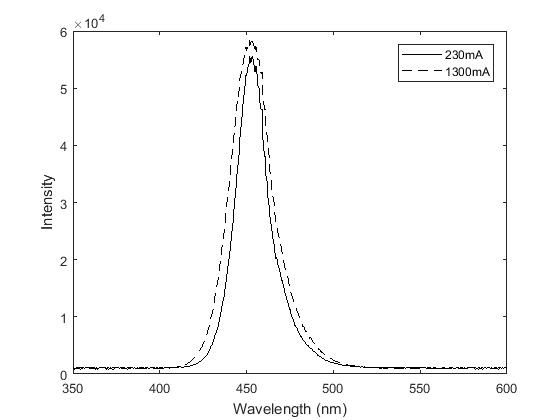
\includegraphics[width=0.6\linewidth]{figures/spektralanalys_mightex455nm}
\caption{Spectrum of the Mightex 455nm \gls{led} using two different driving currents. The band width is slightly wider for the higher current.}
\label{fig:ledspectrum}
\end{figure}

LEDs can sometimes be used with currents far above the specifications, as long as the pulse length is short and the duty cycle is low enough to permit the heat generated to be transported away between the pulses. However, driving the LED with a currents above the specification may affect the efficiency and aging of the LED. LED emittance also depends on the temperature. Depending on the capacitance of the diode, the rise time may limit the current, although there are techniques to shorten the LED pulses \cite{tanaka2011,vele2007}.

The \gls{led} used was fully functional after four months of measurements using a current in the short flashes that was 12 times higher than the maximum continous current specified by the manufacturer. At 12 ampere driving current, the flash duration could be lowered to approximately 250 ns, still using the normal settings of amplification in the camera. The LED was not tested in higher currents, but it seems possible that it could work. A question is how much current the LED can handle, and how its lifetime is affected by higher driving currents.

\section{Statistics}

A value of both \gls{lwc} and \gls{mvd} can be derived from a series of images and since the number of measured droplets will depend on the concentration, the accuracy and precision will depend on the number of samples from the total population of droplets. 

In Paper I, we made an estimation of the precision an instrument could have using the most ideal scenario, where the ``distribution'' was simulated using a single dot of a known size, measured multiple times. This can be seen as a measure of the highest possible precision, defined by the physical limitations of the system components. The coefficient of variation for the LWC was estimated to 1.6 percent for droplets 25 µm in diameter, and 2.4 percent for droplets 10 µm in diameter. In practice it is difficult to compare this with the measured LWC from a real  distribution of droplets. To know the exact LWC, and measure the same content is practically impossible. 

In Paper III, a comparison is made by measuring polymer microspheres in distributions calibrated by NIST. As can be seen in \Cref{tab:poly_meas}, the difference between the measured mean diameter and the stated mean diameter is small. This proves that the size measurement is accurate. It was not possible to estimate the concentration of measured microspheres with the method we used. Possibly, a known concentration could be produced in a water dispersion, but then the optical ambient conditions would also be different.


\section{Droplet Size and Distributions}

Droplets that are very close are likely to coalesce, thereby decreasing the number concentration at a rate that appears to increase for larger droplets and more complex \gls{dsd} \cite{borda2011}. 

Due to the small depth of the measurement volume, i.e. the measuring range compared with the field of view, the likelihood of finding two droplets very close in the image is very low due to the low number concentration of droplets we are measuring. A solution could be to measure the droplet’s circularity and add this as selection criteria for the measurement. This solution also works as a filter for ice or snow particles. 

The \gls{dsd} of cloud droplets 3-50 µm in diameter has usually been considered to follow a lognormal or gamma curve \cite{miles2000,lee2010,sein1998}. This also applies to rain \cite{ulb1983}. However, more recent measurements of \gls{dsd}s show that the distributions greatly varies \cite{james2001,shaw2002,peters2005,cob2011}. Consequently, the results will depend on the measurement method and the sampling volume.

\subsection{Sampling Speed and Measurement Volume}

Since the DII has no external trigger for the imaging, the sampling speed, i.e. the volume of air and droplets that is scanned per time unit, depends on the measuring volume of each image and the imaging speed. 

The sampling speed of the CDP is linearly dependent on the wind speed. The sample area also depends on the size of the measured droplets, but the factory calibration value is given for all sizes. The sampling speed of the DII depends primarily on the image frame rate and the measurement range for each droplet size. At a wind speed of 2 m/s, the sampling speed of the CDP is $\mathrm{4.1 \cdot 10^{-7} m^{3} \cdot s^{-1}}$. This is 39 times higher than the sampling speed of the DII for 20 µm particles. To achieve the same sampling speed, the frame rate of the DII would need to be almost 200 $s^{-1}$. 

Despite the relatively low sampling speed and the small sampling volume of the DII, it seems that by averaging the LWC and the MVD over a period of 30 minutes, enough precision is achieved to be able to compare the two instruments. Since the purpose of the DII is primarily to detect conditions for icing on wind turbines, and provide in-situ observational data for NWP models, the achieved sampling speed may even be good enough, at least for the latter. If the speed is good enough to decide when to switch on de-icing on the blades depends on how quickly the ice builds up, and what de-icing method is used. During icing, high LWC and high MVD are expected.

When comparing the 30 min moving average values for the period 28 February -- 1 March, shown in \Cref{fig:0228-0301_LWCvstime} and \Cref{fig:0228-0301_MVDvstime}, there is very good agreement between the curves, with the exception of 11.30-12.00 when at least ten droplets 25-35 um in diameters were measured by the DII, resulting in a significantly higher MVD and LWC measured by the DII than the CDP. The reason why the CDP did not measure any similarly sized particles on this particular occasion is not known. There is also a difference in the MVD when the LWC is very low resulting in a small number of measured droplets.

The sampling speed could be raised by e.g. changing the optical magnification, but then at the cost of a lower optical resolving power. It could also be increased by raising the output power of the LED, as discussed in \Cref{sec:discnoise} and \Cref{sec:ledillumination}. 

Another way of increasing the sampling speed is to increase the imaging speed. There are cameras with a high imaging speed, and the flash pulse is so short that it would still be a low duty cycle for the LED. The most limiting factor is problably the processing time. This can be solved by implementing parts of the image processing in hardware.

Ideas to increase the sampling speed of the DII are also discussed in the attached papers. 

Finally, the speed requirement depends on the application. If the instrument is used for the verification of NWP models, the sampling speed of the prototype may be enough. If the instrument is to be used for trigger de-icing, the sampling speed may need to be increased.

\subsection{Large Droplets}

Large droplets are important to understand the total size distribution of liquid water droplets and may play an important role during icing. The CDP does not measure particles larger than 50 µm. But if the \gls{dsd} followed a lognormal, or gamma curve \cite{miles2000,lee2010} also for particles larger than 50 µm, enough large droplets should have been detected by the CDP to see an increase in the measured MVD. As demonstrated, this was not always the case. A possible explanation is that the larger cloud droplets do not follow the lognormal distribution when they are above a certain size. If this is true, the predicted MVD may be less useful for the description of a cloud \gls{dsd}, as well as for conclusions about possible icing. In the case with supercooled large droplets, the LWC may be more important to measure than the MVD. But to fully understand this, a parallel measurement using an ice load instrument is required.

\Cref{fig:170505_0441_droplet} and Figure \Cref{fig:170505_1648_droplet} show supercooled large droplets measured during the fog on 05-02-2017.

\begin{figure}[ht]
  \centering
  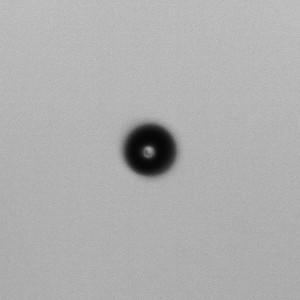
\includegraphics[width=0.4\linewidth]{figures/170205_0441_droplet_74um}
\caption{A 74 µm droplet detected at 04:41 on 05-02-2017.}
\label{fig:170505_0441_droplet}
\end{figure}
\begin{figure}[ht]
  \centering
  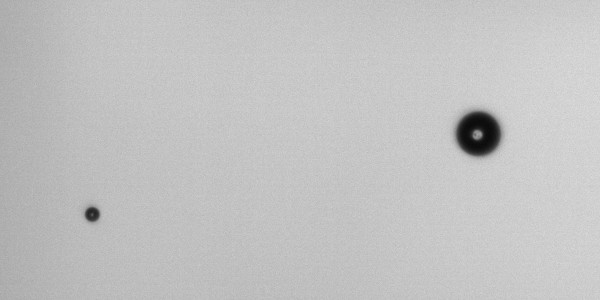
\includegraphics[width=0.8\linewidth]{figures/170205_1648_droplet_19and62um}
\caption{Two droplets, 19 and 62 µm in diameter detected in the same image at 16:48 on 05-02-2017.}
\label{fig:170505_1648_droplet}
\end{figure}


\section{Icing}

The risk of icing increases with increasing wind speed \cite{makk2000}.

During the field study there were several instances when the LWC and MVD was high enough to lead to icing. A study to further investigate the connection between these parameters and the ice load according to ISO 12494 \cite{makk2014} should be carried out. An ice monitoring device, like the Combitech IceMonitor \cite{cost727,thors2015} can be used for this. This should preferably be done in combination with a third independent LWC and MVD measurement, e.g. by using rotating cylinders \cite{makk1992,knez2005}. A heated hygrometer measuring the \gls{twc} can be used as an alternative verification of the LWC measurement when all the atmospheric water is in liquid form \cite{spie2012}.






